% Options for packages loaded elsewhere
\PassOptionsToPackage{unicode}{hyperref}
\PassOptionsToPackage{hyphens}{url}
\PassOptionsToPackage{dvipsnames,svgnames*,x11names*}{xcolor}
%
\documentclass[
  10pt,
]{article}
\usepackage{lmodern}
\usepackage{setspace}
\usepackage{amssymb,amsmath}
\usepackage{ifxetex,ifluatex}
\ifnum 0\ifxetex 1\fi\ifluatex 1\fi=0 % if pdftex
  \usepackage[T1]{fontenc}
  \usepackage[utf8]{inputenc}
  \usepackage{textcomp} % provide euro and other symbols
\else % if luatex or xetex
  \usepackage{unicode-math}
  \defaultfontfeatures{Scale=MatchLowercase}
  \defaultfontfeatures[\rmfamily]{Ligatures=TeX,Scale=1}
  \setmainfont[]{DejaVu Serif}
  \setmonofont[]{DejaVu Sans Mono}
\fi
% Use upquote if available, for straight quotes in verbatim environments
\IfFileExists{upquote.sty}{\usepackage{upquote}}{}
\IfFileExists{microtype.sty}{% use microtype if available
  \usepackage[]{microtype}
  \UseMicrotypeSet[protrusion]{basicmath} % disable protrusion for tt fonts
}{}
\makeatletter
\@ifundefined{KOMAClassName}{% if non-KOMA class
  \IfFileExists{parskip.sty}{%
    \usepackage{parskip}
  }{% else
    \setlength{\parindent}{0pt}
    \setlength{\parskip}{6pt plus 2pt minus 1pt}}
}{% if KOMA class
  \KOMAoptions{parskip=half}}
\makeatother
\usepackage{xcolor}
\IfFileExists{xurl.sty}{\usepackage{xurl}}{} % add URL line breaks if available
\IfFileExists{bookmark.sty}{\usepackage{bookmark}}{\usepackage{hyperref}}
\hypersetup{
  colorlinks=true,
  linkcolor=red,
  filecolor=red,
  citecolor=red,
  urlcolor=red,
  pdfcreator={LaTeX via pandoc}}
\urlstyle{same} % disable monospaced font for URLs
\usepackage[margin=1cm,top=1cm,bottom=1cm,left=1cm,right=1cm,includeheadfoot]{geometry}
\usepackage{listings}
\newcommand{\passthrough}[1]{#1}
\lstset{defaultdialect=[5.3]Lua}
\lstset{defaultdialect=[x86masm]Assembler}
\usepackage{graphicx}
\makeatletter
\def\maxwidth{\ifdim\Gin@nat@width>\linewidth\linewidth\else\Gin@nat@width\fi}
\def\maxheight{\ifdim\Gin@nat@height>\textheight\textheight\else\Gin@nat@height\fi}
\makeatother
% Scale images if necessary, so that they will not overflow the page
% margins by default, and it is still possible to overwrite the defaults
% using explicit options in \includegraphics[width, height, ...]{}
\setkeys{Gin}{width=\maxwidth,height=\maxheight,keepaspectratio}
% Set default figure placement to htbp
\makeatletter
\def\fps@figure{htbp}
\makeatother
\setlength{\emergencystretch}{3em} % prevent overfull lines
\providecommand{\tightlist}{%
  \setlength{\itemsep}{0pt}\setlength{\parskip}{0pt}}
\setcounter{secnumdepth}{3}
% Enable graphics inclusion and ensure figure numbering works
\usepackage{graphicx}
\renewcommand{\figurename}{Figure}

% Configure fonts for Unicode support with fallbacks
\usepackage{newunicodechar}
\newunicodechar{⁴}{\textsuperscript{4}}
\newunicodechar{₄}{\textsubscript{4}}

% Enhanced code block styling for better contrast and readability
\usepackage{fancyvrb}
\usepackage{xcolor}
\usepackage{listings}

% Define custom colors for code blocks
\definecolor{codebg}{RGB}{245, 245, 245}      % Light gray background
\definecolor{codeborder}{RGB}{200, 200, 200}  % Medium gray border
\definecolor{codefg}{RGB}{50, 50, 50}         % Dark gray text

% Configure Verbatim environment for inline code
\DefineVerbatimEnvironment{Verbatim}{Verbatim}{%
    fontsize=\small,
    frame=single,
    framerule=0.5pt,
    framesep=3pt,
    rulecolor=\color{codeborder},
    bgcolor=\color{codebg},
    fgcolor=\color{codefg}
}

% Configure code block styling
\DefineVerbatimEnvironment{Highlighting}{Verbatim}{%
    fontsize=\footnotesize,
    frame=single,
    framerule=0.5pt,
    framesep=5pt,
    rulecolor=\color{codeborder},
    bgcolor=\color{codebg},
    fgcolor=\color{codefg}
}

% Style inline code with \texttt
\renewcommand{\texttt}[1]{%
    \colorbox{codebg}{\color{codefg}\ttfamily #1}%
}

% Configure listings package for code blocks
\lstset{
    backgroundcolor=\color{codebg},
    basicstyle=\footnotesize\ttfamily\color{codefg},
    breakatwhitespace=false,
    breaklines=true,
    captionpos=b,
    commentstyle=\color{codefg},
    deletekeywords={...},
    escapeinside={\%*}{*)},
    extendedchars=true,
    frame=single,
    framerule=0.5pt,
    framesep=5pt,
    keepspaces=true,
    keywordstyle=\color{codefg},
    language=Python,
    morekeywords={*,...},
    numbers=left,
    numbersep=5pt,
    numberstyle=\tiny\color{codefg},
    rulecolor=\color{codeborder},
    showspaces=false,
    showstringspaces=false,
    showtabs=false,
    stepnumber=1,
    stringstyle=\color{codefg},
    tabsize=2,
    title=\lstname
}

% Override any Pandoc default lstset configurations
\AtBeginDocument{
    \lstset{
        backgroundcolor=\color{codebg},
        basicstyle=\footnotesize\ttfamily\color{codefg},
        frame=single,
        framerule=0.5pt,
        framesep=5pt,
        rulecolor=\color{codeborder},
        numbers=left,
        numbersep=5pt,
        numberstyle=\tiny\color{codefg}
    }
}

% Configure hyperref colors consistently
\AtBeginDocument{
% Override pandoc's hidelinks setting with consistent options
\hypersetup{
    colorlinks=true,
    allcolors=red,
    linkcolor=red,
    urlcolor=red,
    citecolor=red,
    filecolor=red,
    menucolor=red,
    linktoc=all
}
}

% Simple page break support for document structure
% Note: Page breaks are handled in the markdown generation, not here

\title{Introduction}
\author{Daniel Ari Friedman\\ ORCID: 0000-0001-6232-9096\\ Email: daniel@activeinference.institute}
\date{August 15, 2025}

\begin{document}
\maketitle

{
\hypersetup{linkcolor=black}
\setcounter{tocdepth}{3}
\tableofcontents
}
\setstretch{1.0}
\hypertarget{introduction}{%
\section{Introduction}\label{introduction}}

Quadray coordinates provide a tetrahedral basis for modeling space and
computation, standing in contrast to Cartesian cubic frameworks.
Originating in Buckminster Fuller's Synergetics, quadray coordinates
enable the replacement of right-angle orthonormal assumptions, with
60-degree coordination and a unit tetrahedron of volume 1. This
reframing yields striking integer relationships among common polyhedra
and provides a natural account of space via close-packed spheres and the
isotropic vector matrix (IVM).

In this synthetic review, we distinguish three internal meanings of
``4D,'' following a dot-notation that avoids cross-domain confusion:

\begin{itemize}
\tightlist
\item
  \textbf{Coxeter.4D} --- four-dimensional Euclidean space (E⁴), as in
  classical polytope theory. Coxeter emphasizes that Euclidean 4D is not
  spacetime; see the Dover edition of Regular Polytopes (p.~119) for a
  clear statement to this effect; background on lattice packings in four
  dimensions aligns with the treatment in Conway \& Sloane's
  \href{https://link.springer.com/book/10.1007/978-1-4757-6568-7}{Sphere
  Packings, Lattices and Groups}.
\item
  \textbf{Einstein.4D} --- Minkowski spacetime (3D + time) with an
  indefinite metric; appropriate for relativistic physics but distinct
  from Euclidean E⁴.
\item
  \textbf{Fuller.4D} --- synergetics' tetrahedral accounting of space
  using Quadrays (four non-negative coordinates with at least one zero
  after normalization) and the Isotropic Vector Matrix (IVM) = Cubic
  Close Packing (CCP) = Face-Centered Cubic (FCC) correspondence. This
  treats the regular tetrahedron as a natural unit container and
  emphasizes angle/shape relations independent of time/energy.
\end{itemize}

This paper unifies three threads:

\begin{itemize}
\tightlist
\item
  \textbf{Foundations}: Quadray coordinates and their relation to 4D
  modeling more generally, with explicit namespace usage (Coxeter.4D,
  Einstein.4D, Fuller.4D) to maintain clarity.
\item
  \textbf{Optimization framework}: leverages integer volume quantization
  on tetrahedral lattices to achieve robust, discrete convergence.
\item
  \textbf{Information geometry}: tools (e.g., Fisher Information,
  free-energy minimization) for interpreting optimization as geodesic
  motion on statistical manifolds.
\end{itemize}

Contributions:

\begin{itemize}
\tightlist
\item
  \textbf{Namespaces mapping}: Coxeter.4D (Euclidean E⁴), Einstein.4D
  (Minkowski spacetime), and Fuller.4D (Quadrays/IVM) → analytical tools
  and examples.
\item
  \textbf{Quadray-adapted Nelder--Mead}: integer-lattice normalization
  and volume-level tracking.
\item
  \textbf{Equations and methods}: comprehensive supplement with guidance
  for high-precision computation using
  \passthrough{\lstinline!libquadmath!}.
\item
  \textbf{Discrete optimizer}: integer-valued variational descent over
  the IVM (\passthrough{\lstinline!discrete\_ivm\_descent!}) with
  animation tooling, connecting lattice geometry to
  information-theoretic objectives.
\end{itemize}

\hypertarget{companion-code-and-tests}{%
\subsection{Companion code and tests}\label{companion-code-and-tests}}

The manuscript is accompanied by a fully-tested Python codebase under
\passthrough{\lstinline!src/!} with unit tests under
\passthrough{\lstinline!tests/!}. Key artifacts used throughout the
paper:

\begin{itemize}
\tightlist
\item
  \textbf{Quadray APIs}: \passthrough{\lstinline!src/quadray.py!}
  (\passthrough{\lstinline!Quadray!},
  \passthrough{\lstinline!integer\_tetra\_volume!},
  \passthrough{\lstinline!ace\_tetravolume\_5x5!}).
\item
  \textbf{Determinant utilities}:
  \passthrough{\lstinline!src/linalg\_utils.py!}
  (\passthrough{\lstinline!bareiss\_determinant\_int!}).
\item
  \textbf{Length-based volume}:
  \passthrough{\lstinline!src/cayley\_menger.py!}
  (\passthrough{\lstinline!tetra\_volume\_cayley\_menger!},
  \passthrough{\lstinline!ivm\_tetra\_volume\_cayley\_menger!}).
\item
  \textbf{XYZ conversion}: \passthrough{\lstinline!src/conversions.py!}
  (\passthrough{\lstinline!urner\_embedding!},
  \passthrough{\lstinline!quadray\_to\_xyz!}).
\item
  \textbf{Examples}: \passthrough{\lstinline!src/examples.py!}
  (\passthrough{\lstinline!example\_ivm\_neighbors!},
  \passthrough{\lstinline!example\_volume!},
  \passthrough{\lstinline!example\_optimize!}).
\end{itemize}

For comprehensive background resources, computational implementations,
and related work, see the \href{07_resources.md}{Resources} section.

Graphical abstract: Panel A shows Quadray axes (A,B,C,D) under a
symmetric embedding with wireframe context. Panel B shows close-packed
spheres at the tetrahedron vertices (IVM/CCP/FCC, ``twelve around
one'').

\begin{figure}
\centering
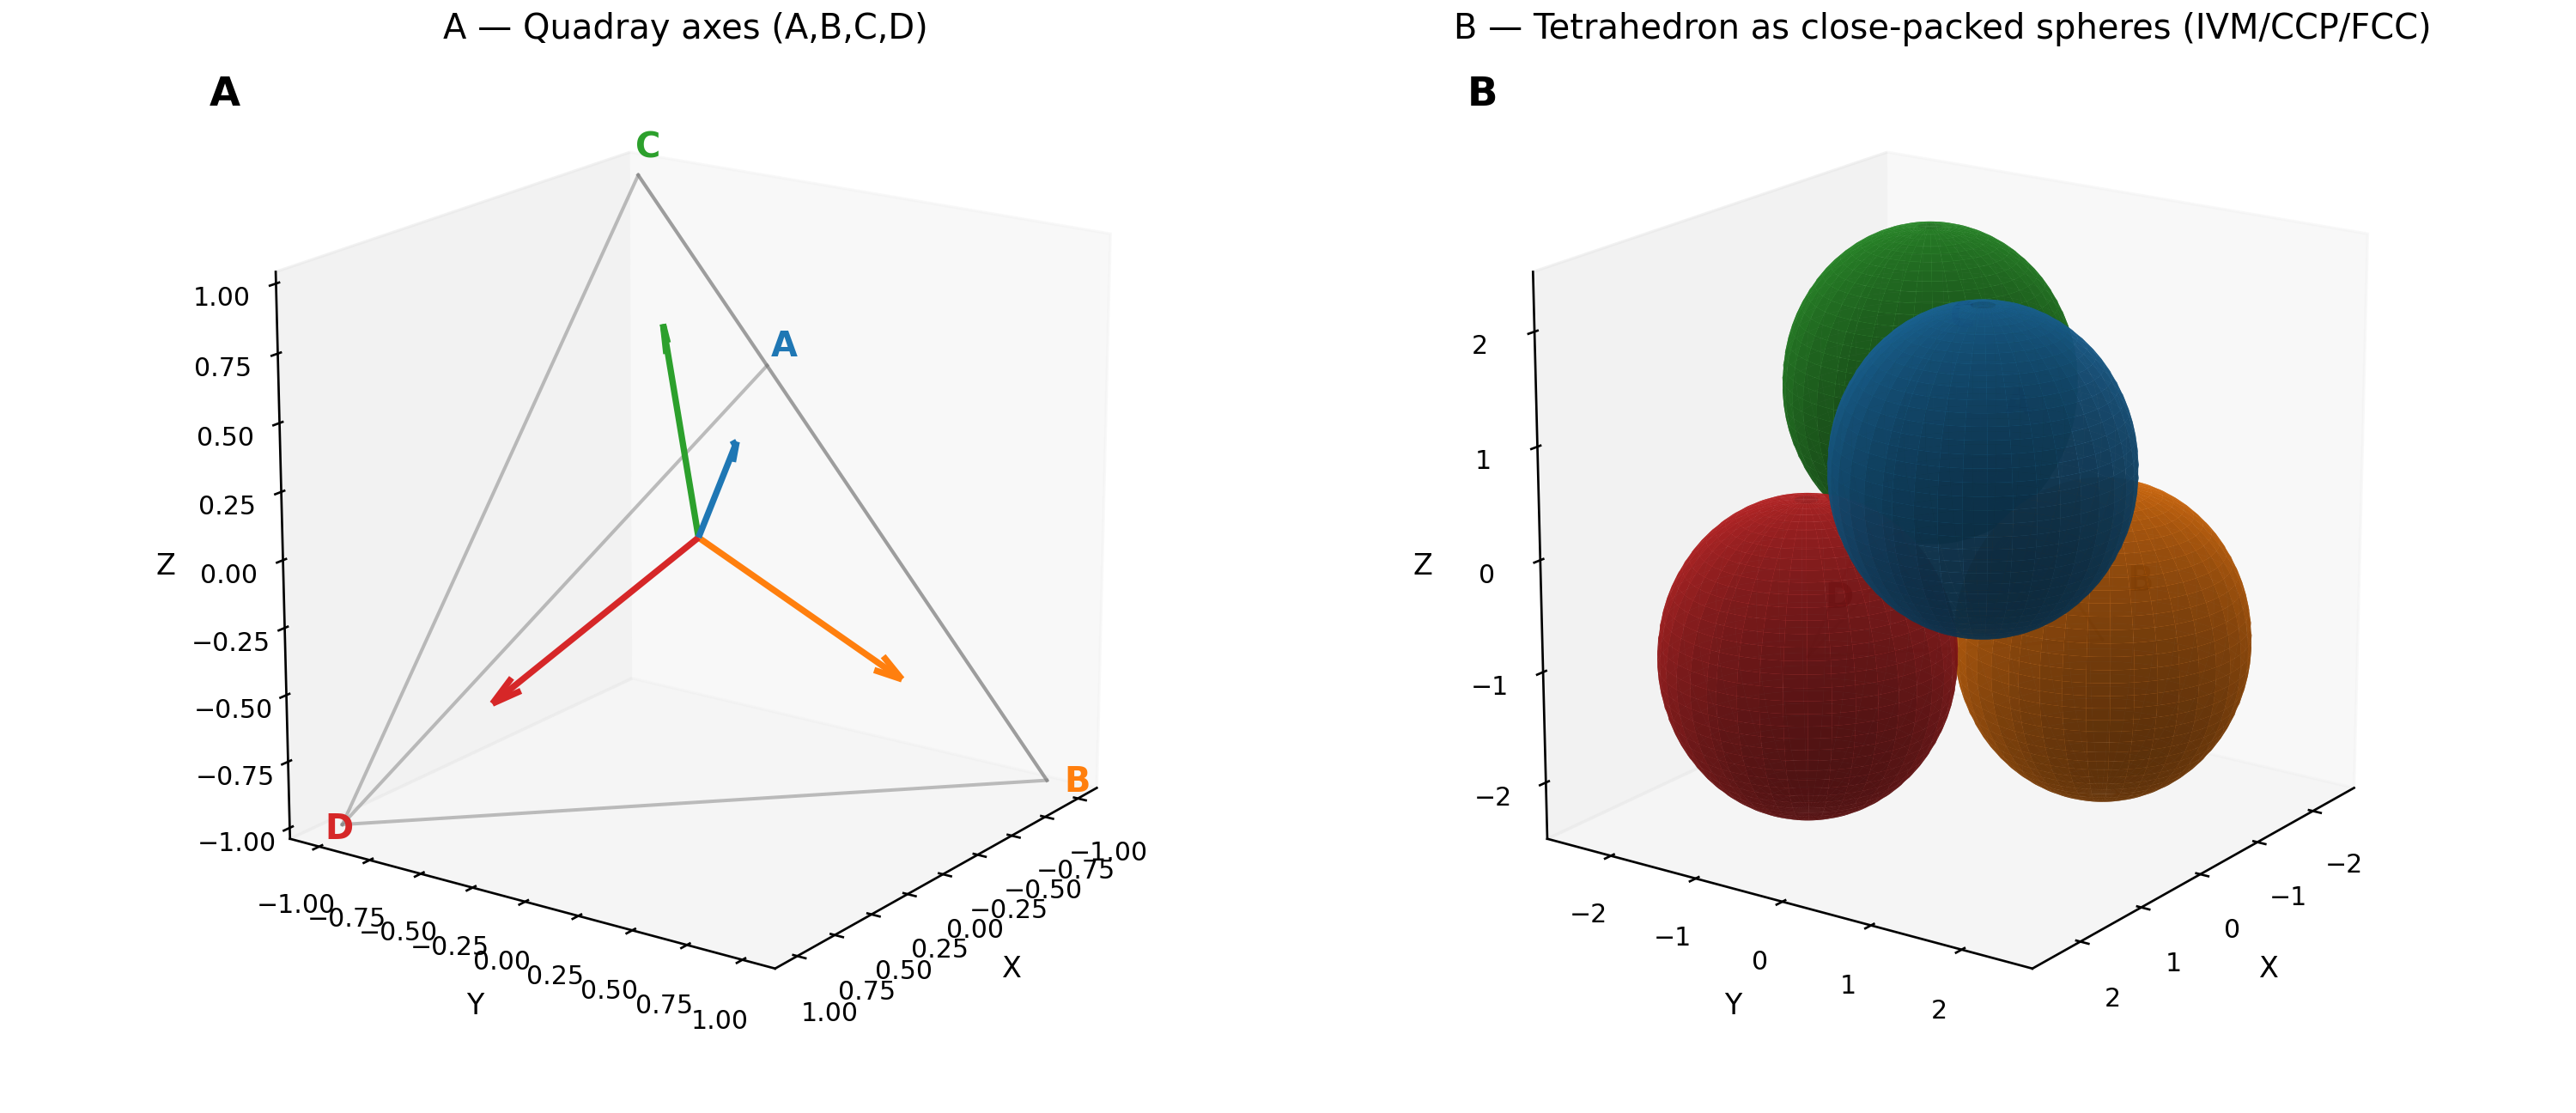
\includegraphics{../output/figures/graphical_abstract_quadray.png}
\caption{\textbf{Quadray coordinate system overview (graphical
abstract)}. \textbf{Panel A}: Four Quadray axes (A,B,C,D) rendered as
colored directional arrows from the origin to the vertices of a regular
tetrahedron under the default symmetric embedding. Each axis is
distinctly colored (A=blue, B=orange, C=green, D=red) with axis labels
positioned at the vertex endpoints. A light gray wireframe connects the
four vertices to emphasize the tetrahedral geometry underlying the
coordinate system. This panel illustrates the fundamental Fuller.4D
direction-based structure where Quadrays represent four canonical
directions in tetrahedral space rather than orthogonal Cartesian
dimensions. \textbf{Panel B}: The same tetrahedral vertices shown as
close-packed spheres with radius chosen so neighboring spheres kiss
along tetrahedron edges, emphasizing the connection to the Isotropic
Vector Matrix (IVM), Cubic Close Packing (CCP), and Face-Centered Cubic
(FCC) arrangements. Each sphere is colored to match its corresponding
axis from Panel A, with light edge wireframes providing geometric
context. This visualization demonstrates how Quadray coordinates
naturally align with dense sphere packing and the ``twelve around one''
coordination motif central to synergetics and Fuller.4D modeling.}
\end{figure}

\end{document}
